\documentclass[10pt]{article}

\usepackage[margin=1in]{geometry}
\usepackage[T1]{fontenc}
\usepackage{lmodern}
\usepackage{microtype}
\usepackage{amsmath,amssymb}
\usepackage{booktabs}
\usepackage{array}
\usepackage{multirow}
\usepackage{graphicx}
\usepackage{tikz}
\usetikzlibrary{arrows.meta,positioning}
\usepackage{pgfplots}
\pgfplotsset{compat=1.18}
\usepackage{natbib}
\usepackage{hyperref}
\usepackage{xurl}

\title{When Missing Evidence Leaves No Trace:\\
Obligation Coverage and Silent Retrieval Failures in Agent Decision Safety}

\author{Anonymous Authors}

\date{}

% Auto-transcribed from frozen P2 results.
% Source: research/evidence-surface-v1/p2/out/p2-results.json
% Frozen blob SHA: e8a749a6707dbf4614b20ef6248f81eb43dd89d4
% Do not edit values by hand without reconciling against the frozen JSON.

\newcommand{\PtwoN}{180}
\newcommand{\PtwoEvaluations}{1080}
\newcommand{\CzeroUnsupported}{0}
\newcommand{\ConeUnsupported}{30}
\newcommand{\CzeroUDR}{0.00}
\newcommand{\ConeUDR}{16.67}
\newcommand{\PrimaryRD}{16.67}
\newcommand{\PrimaryCILow}{11.67}
\newcommand{\PrimaryCIHigh}{22.22}
\newcommand{\PrimaryP}{1.8626451492309587\times 10^{-9}}

\newcommand{\LexRecall}{63.06}
\newcommand{\HashRecall}{57.22}
\newcommand{\HybridRecall}{60.00}

\newcommand{\LexUDR}{31.11}
\newcommand{\HashUDR}{33.89}
\newcommand{\HybridUDR}{29.44}
\newcommand{\CoverageUDR}{0.00}

\newcommand{\LexCoverage}{53.33}
\newcommand{\HashCoverage}{47.78}
\newcommand{\HybridCoverage}{51.67}
\newcommand{\CoverageCoverage}{51.67}

\newcommand{\LexDecisive}{84.44}
\newcommand{\HashDecisive}{81.67}
\newcommand{\HybridDecisive}{81.11}
\newcommand{\CoverageDecisive}{51.67}

\newcommand{\LexSafeDecisive}{53.33}
\newcommand{\HashSafeDecisive}{47.78}
\newcommand{\HybridSafeDecisive}{51.67}
\newcommand{\CoverageSafeDecisive}{51.67}

\newcommand{\HybridFallback}{18.89}
\newcommand{\CoverageFallback}{48.33}
\newcommand{\HybridCompleteCount}{93}

% Direct C1 family UDR (%)
\newcommand{\FoneCOne}{0}
\newcommand{\FtwoCOne}{0}
\newcommand{\FthreeCOne}{0}
\newcommand{\FfourCOne}{0}
\newcommand{\FfiveCOne}{0}
\newcommand{\FsixCOne}{100}

% Retrieval family UDR (%): Lexical / Hash-dense / Hybrid / Coverage-aware
\newcommand{\FoneLex}{66.67}
\newcommand{\FoneHash}{86.67}
\newcommand{\FoneHybrid}{70.00}
\newcommand{\FoneCoverage}{0}

\newcommand{\FtwoLex}{40.00}
\newcommand{\FtwoHash}{26.67}
\newcommand{\FtwoHybrid}{6.67}
\newcommand{\FtwoCoverage}{0}

\newcommand{\FthreeLex}{0}
\newcommand{\FthreeHash}{0}
\newcommand{\FthreeHybrid}{0}
\newcommand{\FthreeCoverage}{0}

\newcommand{\FfourLex}{20.00}
\newcommand{\FfourHash}{13.33}
\newcommand{\FfourHybrid}{20.00}
\newcommand{\FfourCoverage}{0}

\newcommand{\FfiveLex}{0}
\newcommand{\FfiveHash}{0}
\newcommand{\FfiveHybrid}{0}
\newcommand{\FfiveCoverage}{0}

\newcommand{\FsixLex}{60.00}
\newcommand{\FsixHash}{76.67}
\newcommand{\FsixHybrid}{80.00}
\newcommand{\FsixCoverage}{0}


\begin{document}
\maketitle

\begin{abstract}
Decision-capable agents often rely on retrieved evidence before taking consequential actions.
Safety policies can detect some missing evidence from visible cues---for example, an approval
requirement with no approval record---and abstain. Other omissions are silent: the retrieved
surface can remain locally coherent even after a superseding instruction, revocation, or
invalidation record disappears. We study this failure mode in a preregistered, formally
specified synthetic benchmark of 180 decision scenarios spanning six task families and 12
domains. Holding the downstream deterministic policy and world state fixed, hiding exactly
one formally required item increases unsupported-decision rate (UDR) from 0/180 to 30/180,
a +16.67 percentage-point paired risk difference (95\% bootstrap CI [11.67, 22.22];
exact two-sided McNemar $p=1.86\times10^{-9}$). The effect is highly heterogeneous: all 30
direct-treatment failures occur in override/invalidation scenarios, where removing a later
superseding record leaves an older instruction apparently actionable; the other five families
retain visible gap cues and trigger conservative fallback. Across three frozen top-$k$
retrievers, UDR ranges from 29.44\% to 33.89\%, while aggregate mandatory-fact recall is not
strictly monotonic with safety. Finally, on the identical frozen hybrid retrieval surface,
adding only a one-bit evidence-obligation completeness signal reduces UDR from 29.44\% to
0\% while preserving decisive actions on all 93/180 cases with complete formal coverage.
The results isolate a distinction between missing evidence and \emph{undetectably} missing
evidence: retrieval quality matters, but downstream safety also depends on whether the policy
can know that a required obligation is uncovered.
\end{abstract}


\section{Introduction}
\label{sec:intro}

Long-horizon agents increasingly act over state assembled from memory, retrieval, tools,
logs, and prior decisions. The downstream decision policy rarely sees the entire underlying
world state. Instead, it sees a \emph{decision-visible evidence surface}: a finite set of
records selected by upstream retrieval and filtering stages.

This creates a safety problem that ordinary relevance metrics do not fully capture. A
policy can be conservative when missing information is itself visible. If an approval
requirement remains visible but the approval record is absent, the policy can request
approval. If a stale record is visible without a current replacement, the policy can
defer. If two claims conflict and no resolution record is present, the policy can clarify.
We call these \emph{detectable gaps}.

A different failure occurs when evidence loss removes both a required item and the only
cue that anything is missing. Consider an earlier instruction to execute an action followed
by a later override cancelling it. If retrieval drops the cancellation, the remaining
surface can contain a coherent older instruction plus readiness evidence. A downstream
policy that checks only what it can see has no local signal that a later override exists.
We call this a \emph{silent evidence omission}.

\begin{figure}[t]
\centering
\resizebox{\linewidth}{!}{% Conceptual figure: no empirical data.
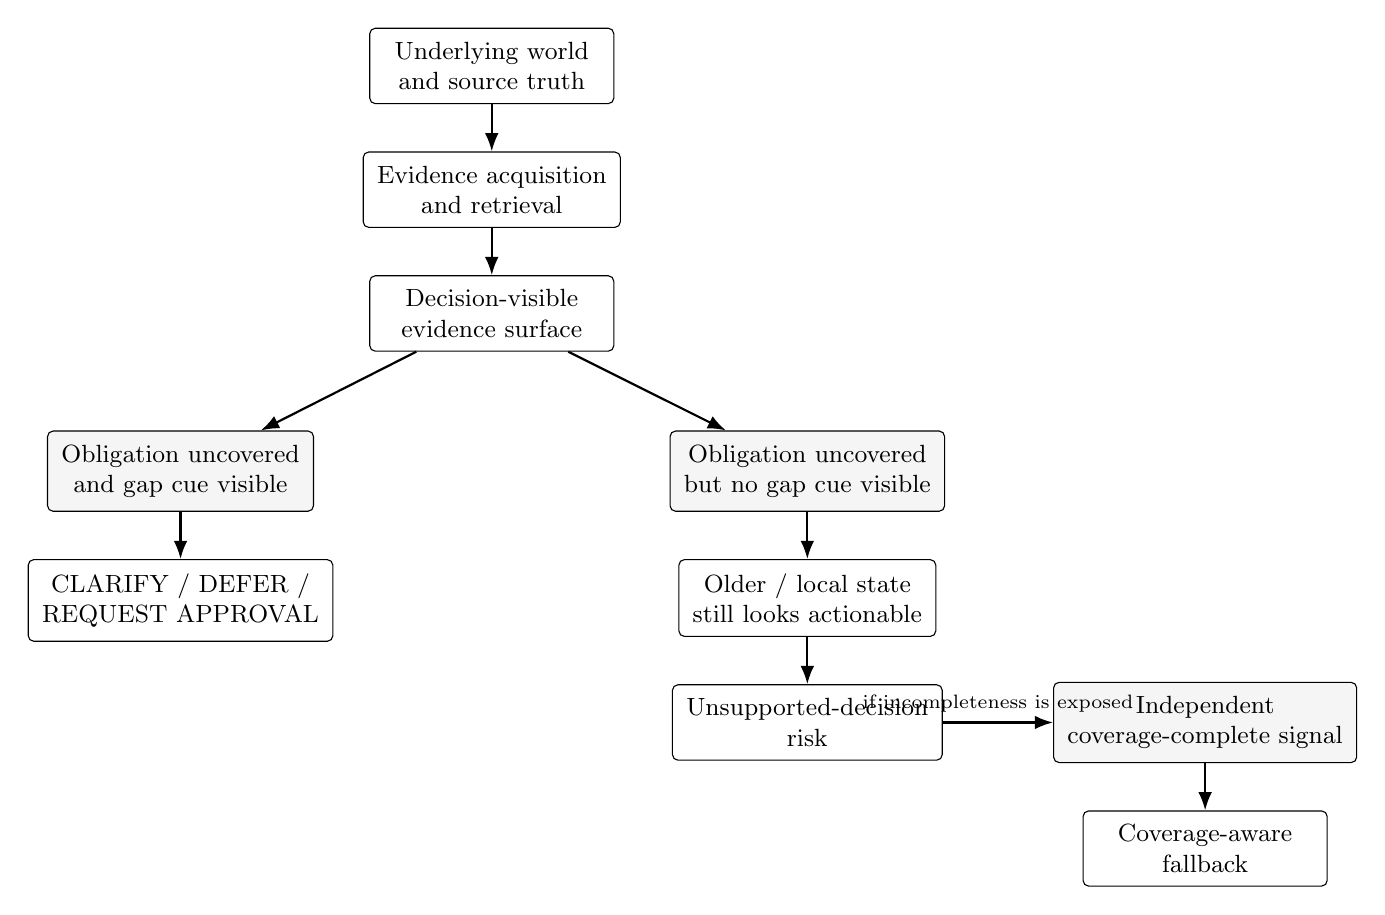
\begin{tikzpicture}[
  node distance=6mm and 7mm,
  every node/.style={font=\small},
  box/.style={draw, rounded corners=2pt, align=center, inner sep=5pt, minimum width=31mm},
  decision/.style={draw, rounded corners=2pt, align=center, inner sep=5pt, minimum width=32mm, fill=black!4},
  arrow/.style={-Latex, thick}
]
\node[box] (world) {Underlying world\\and source truth};
\node[box, below=of world] (retrieval) {Evidence acquisition\\and retrieval};
\node[box, below=of retrieval] (surface) {Decision-visible\\evidence surface};

\node[decision, below left=10mm and 7mm of surface] (visible) {Obligation uncovered\\and gap cue visible};
\node[decision, below right=10mm and 7mm of surface] (silent) {Obligation uncovered\\but no gap cue visible};

\node[box, below=of visible] (fallback) {CLARIFY / DEFER /\\REQUEST APPROVAL};
\node[box, below=of silent] (unsafe) {Older / local state\\still looks actionable};

\node[box, below=of unsafe] (risk) {Unsupported-decision\\risk};
\node[decision, right=14mm of risk] (coverage) {Independent\\coverage-complete signal};
\node[box, below=of coverage] (safe2) {Coverage-aware\\fallback};

\draw[arrow] (world) -- (retrieval);
\draw[arrow] (retrieval) -- (surface);
\draw[arrow] (surface) -- (visible);
\draw[arrow] (surface) -- (silent);
\draw[arrow] (visible) -- (fallback);
\draw[arrow] (silent) -- (unsafe);
\draw[arrow] (unsafe) -- (risk);
\draw[arrow] (risk) -- node[above, font=\scriptsize]{if incompleteness is exposed} (coverage);
\draw[arrow] (coverage) -- (safe2);
\end{tikzpicture}
}
\caption{\textbf{Missing evidence is not a single failure mode.} A downstream policy can
react safely when an uncovered obligation leaves a visible gap cue. A silent omission
removes the required evidence without leaving such a cue. The coverage-aware condition
tests a separate completeness signal without revealing the missing content.}
\label{fig:mechanism}
\end{figure}

This failure is distinct from two nearby problems. STALE studies whether agents revise
state correctly when later evidence is available but implicitly invalidates older memory
\citep{chao2026stale}. Revocation-enforcement work studies the opposite read-path error:
an already revoked record remains retrievable and authoritative
\citep{shen2026revoked}. Our intervention removes the \emph{superseding valid record}
from the decision-visible surface, so the older record can remain locally coherent without
any observable revocation cue.

We ask three questions:
\begin{enumerate}
  \item \textbf{Causal visibility:} does hiding formally required evidence, while holding
  task and policy fixed, increase unsupported decisive behavior?
  \item \textbf{Failure mechanism:} are all missing obligations equally dangerous, or are
  failures concentrated where absence is silent relative to visible-gap checks?
  \item \textbf{Coverage signaling:} can a signal that required obligations are incomplete
  prevent unsupported decisions without revealing the missing content itself?
\end{enumerate}

We study these questions in a preregistered, formally specified synthetic benchmark with
180 scenarios spanning six task families and 12 domains. Each scenario contains a
machine-readable source truth, explicit evidence obligations, rendered evidence, a frozen
decision-safety contract, and paired FULL/HIDDEN treatments. Two separately implemented
formal validators must agree before a sample is admitted.

The confirmatory experiment uses one frozen deterministic downstream policy and six
conditions. C0 exposes all formal evidence. C1 removes exactly one designated mandatory
item. C2--C4 use frozen lexical, hashed-dense, and hybrid top-$k$ retrieval. C5 reuses the
\emph{identical C4 retrieval surface} and adds only a boolean
\texttt{coverage\_complete} signal.

The principal result is not that all missing evidence is dangerous. The paired C0$\to$C1
intervention raises UDR from 0\% to 16.67\%, but all 30 direct-treatment failures occur in
the override/invalidation family. In the other five families, the omission leaves a
policy-visible structural cue and the frozen policy falls back conservatively. Under
ordinary top-$k$ retrieval, however, unsupported decisions also appear in constraint,
authority, and conflict families because retrieval can remove combinations of evidence
or the cue-bearing record itself. Silentness is therefore a property of the
\emph{resulting surface relative to the policy}, not merely a task-family label.

Our contributions are:
\begin{itemize}
  \item a policy-relative formalization of \emph{silent evidence omission}, distinct from
  stale-state resolution and from retrieval that returns explicitly revoked records;
  \item a preregistered paired intervention that holds world state and downstream policy
  fixed while changing mandatory-evidence visibility;
  \item a boundary characterization showing that direct hiding is safe when a visible gap
  remains, but unsafe for superseding override/invalidation evidence whose omission leaves
  an apparently actionable surface;
  \item evidence that aggregate mandatory-fact recall does not induce a strict monotonic
  safety ordering across the frozen retrievers; and
  \item a same-surface mechanism test showing that obligation-completeness information is
  sufficient, under the formal benchmark, to remove the measured unsupported decisions
  without suppressing decisions on complete-coverage cases.
\end{itemize}

Our claims are deliberately narrow. The benchmark is synthetic and formal. It does not
establish human-preference validity, real-world failure prevalence, deployment safety, or
a universal theorem about agents.


\section{Related Work}
\label{sec:related}

\paragraph{Agent memory and retrieval.}
Persistent-agent memory systems study how histories should be stored, retrieved, organized,
and updated. MemGPT treats memory as an external substrate managed across context tiers
\citep{packer2023memgpt}; A-Mem develops linked agentic memory
\citep{xu2025amem}; and Hindsight combines vector, keyword, graph, and temporal retrieval
over structured memory networks \citep{latimer2026hindsight}. Memora evaluates long-term
remembering, reasoning, recommending, and the reuse of invalidated memory
\citep{uddin2026memora}. These systems motivate the long-horizon setting, but our study does
not propose another memory architecture. We treat retrieval as an upstream intervention and
ask how evidence visibility changes downstream supportedness.

\paragraph{Evidence sufficiency, coverage, and selective answering.}
Retrieval relevance is not the same as evidential support. RAG established retrieval as a
grounding mechanism \citep{lewis2020rag}; AbstentionBench shows that even strong reasoning
models struggle to abstain on unanswerable inputs \citep{kirichenko2025abstentionbench}.
SURE-RAG explicitly models whether a delivered evidence set supports, refutes, or is
insufficient for an answer \citep{qiu2026surerag}. HALT frames stopping in search agents as
evidence coverage over expected claims \citep{roh2026halt}, and
Evidence-Obligation Pool-Gated Retrieval uses an explicit obligation ledger and warrant
gate \citep{kim2026obligation}. We therefore do \emph{not} claim novelty for evidence
sufficiency, evidence coverage, or evidence obligations as concepts.

A particularly relevant methodological result is \emph{Before Answering}
\citep{mondal2026before}, which shows that deleting supporting evidence can create a
memory-size shortcut for insufficiency detection. Our benchmark does not train a detector
of treatment status: the frozen policy receives no Gold, treatment label, or expected-count
input. Nevertheless, surface cardinality can differ after removal, so we make the narrower
claim that an omission is \emph{silent relative to the frozen policy's declared gap checks},
not statistically undetectable to every possible classifier.

Our main failure can occur before visible-evidence sufficiency is assessed: the delivered
surface may look locally actionable precisely because the record that would reveal a state
transition, supersession, or invalidation is absent.

\paragraph{Temporal state, belief revision, and revocation.}
Belief revision and truth-maintenance systems formalize how conclusions should change as
evidence changes \citep{alchourron1985logic,doyle1979truth}; temporal reasoning formalizes
validity over time \citep{allen1983maintaining}. STALE studies implicit conflict, where
later observations are available but agents fail to resolve the current state
\citep{chao2026stale}. \citet{shen2026revoked} study revocation enforcement: records already
marked revoked can still be returned, outrank replacements, and drive actions.

Our boundary is complementary. In revocation-enforcement failure, an invalid record is
returned even though revocation/replacement state exists in the memory path. In our
silent-omission intervention, the \emph{superseding valid record itself} is absent from the
decision-visible surface. In STALE, later evidence is available but not correctly
integrated; here, the evidence encoding the transition may never reach the downstream
policy.

\begin{table}[t]
\centering
\small
\setlength{\tabcolsep}{4pt}
\resizebox{\columnwidth}{!}{%
\begin{tabular}{p{0.19\columnwidth}p{0.29\columnwidth}p{0.27\columnwidth}p{0.19\columnwidth}}
\toprule
Work & Primary failure boundary & Updating / revoking evidence & Main direction \\
\midrule
SURE-RAG & Delivered set may be insufficient & Visible set is inspected & Verify / abstain \\
STALE & New evidence does not revise prior state & Later evidence exists & State consolidation \\
Revoked but Still Authoritative & Revoked record is still returned & Revocation exists in memory path & Filter invalid records \\
\textbf{This work} & Superseding evidence disappears without a visible gap & \textbf{Transition evidence absent from decision surface} & \textbf{Obligation coverage} \\
\bottomrule
\end{tabular}%
}
\caption{Functional boundary relative to the nearest contemporary work. The rows address
adjacent failure surfaces and are not intended as a performance ranking.}
\label{tab:nearest}
\end{table}


\section{Problem Formulation}
\label{sec:formal}

For a decision instance $x$, let $O(x)$ be the set of evidence obligations required by a
frozen formal safety contract, and let $S(x)$ be the evidence surface delivered to the
downstream policy.

\paragraph{Formal coverage.}
Define $C(x,S)=1$ iff every obligation in $O(x)$ is covered by $S$, and $C(x,S)=0$
otherwise. Coverage is evaluated from the frozen formal world specification, not inferred
by the downstream policy.

\paragraph{Unsupported decisive behavior.}
Let $a(x,S)$ be the policy action. Actions are partitioned into consequential decisive
actions and safe fallback actions such as \textsc{Clarify}, \textsc{Defer}, or
\textsc{RequestApproval}. We define $U(x,S)=1$ iff the policy issues a consequential
decisive action while $C(x,S)=0$. The unsupported-decision rate (UDR) is the mean of $U$
over a condition. UDR is a contract-level supportedness metric; it is not a human-preference,
utility, or real-world correctness metric.

\paragraph{Detectable gaps and silent omissions.}
Let $G(S)=1$ when the frozen policy's visible-gap checks detect that required information is
missing. An uncovered obligation is \emph{detectable} when $C(x,S)=0$ and $G(S)=1$, causing
a safe fallback. It is \emph{silent relative to the policy} when
\[
C(x,S)=0 \quad \text{and} \quad G(S)=0.
\]
In that case, the delivered surface contains no local cue that a required obligation is
uncovered. The definition is policy-relative: an omission silent for one policy may be
detectable for another.

\begin{table}[t]
\centering
\scriptsize
\setlength{\tabcolsep}{2pt}
\begin{tabular}{p{0.18\columnwidth}p{0.18\columnwidth}p{0.51\columnwidth}}
\toprule
Formal coverage & Visible gap cue & Expected frozen-policy behavior \\
\midrule
Complete & irrelevant & decisive action may be supported \\
Incomplete & present & safe fallback \\
Incomplete & absent & silent-omission risk \\
Incomplete + coverage signal & may be absent & coverage-aware fallback \\
\bottomrule
\end{tabular}
\caption{Mechanism taxonomy. This is a property of the formal contract and frozen policy,
not a claim that all deployed agents implement the same gap checks.}
\label{tab:taxonomy}
\end{table}

\paragraph{Coverage-completeness signal.}
C5 augments the policy input with one boolean $z=C(x,S)$. No missing evidence content is
disclosed. If $z=0$, the frozen C5 rule returns \textsc{Defer} before the ordinary policy
logic. If $z=1$, it executes the same logic as the coverage-blind conditions. C5 is
therefore a mechanism test: it asks whether making obligation incompleteness observable is
sufficient to prevent the measured unsupported-decision failure on an otherwise identical
surface.


\section{Benchmark and Experimental Design}
\label{sec:method}

\subsection{Fresh formal benchmark}

We construct 180 fresh scenarios: six task families with 30 samples each, distributed
across 12 domains. Each sample contains a machine-readable \texttt{world\_spec}, source
records with timestamps and provenance, a rendered decision question, distractor evidence,
explicit required facts, permissible action families, and a safe fallback when obligations
are uncovered.

\begin{table}[t]
\centering
\small
\setlength{\tabcolsep}{4pt}
\begin{tabular}{p{0.08\linewidth}p{0.23\linewidth}p{0.31\linewidth}p{0.30\linewidth}}
\toprule
Family & Obligation & C1 visible-gap cue & Silent-failure route \\
\midrule
F1 & Constraint / feasibility & Requirement remains while feasibility support is missing & Top-$k$ can remove cue-bearing context together with support \\
F2 & Authority / approval & Authority requirement remains without current grant & Top-$k$ can surface action support without the requirement \\
F3 & Temporal validity & Stale marker remains without current replacement & Not observed under frozen retrievers \\
F4 & Conflict resolution & Conflicting claims remain without resolution & Top-$k$ can remove one side or the resolution structure \\
F5 & Outcome / revision & Prior conditional decision remains without change evidence & Not observed under frozen retrievers \\
F6 & Override / invalidation & None when later override is removed & Older instruction remains locally actionable \\
\bottomrule
\end{tabular}
\caption{Task families and policy-relative gap structure. The last column describes a
possible silent surface under the frozen policy; it is not a universal property of the
family.}
\label{tab:families}
\end{table}

The benchmark is independent of the earlier TMLR validation benchmark and sealed Holdback;
neither is reused as confirmatory evidence here.

\subsection{Formal validation and freeze}

Every formal sample must pass two separately implemented validators:
(1) a declarative evaluator reading the frozen \texttt{world\_spec.decision\_contract};
and (2) a family-specific evaluator that independently derives required fact types and
action families. They must agree exactly on required fact IDs, mandatory evidence IDs,
full-evidence action families, fallback action families, and coverage completeness.

Each sample also passes metamorphic controls:
FULL covers every required obligation; hiding the designated treatment target makes at
least one required obligation uncovered; removing a declared non-mandatory evidence item
preserves complete coverage; and world truth is unchanged across the paired treatment.

Before P2, the frozen dataset had zero schema failures, zero dual-validator disagreements,
zero renderer/world-spec consistency failures, zero dataset-audit errors, and zero
near-duplicate warnings.

\subsection{Frozen downstream policy}

P2 uses one deterministic policy frozen before outcomes. In C0--C4 it can read only the
decision question, visible evidence role, evidence currentness, candidate support,
candidate actions, and prior-state fields. It cannot read \texttt{world\_spec}, Gold,
condition labels, treatment targets, or construction metadata.

Its visible-gap rules are frozen as:
\begin{itemize}
  \item visible constraint requirement with no feasibility evidence $\rightarrow$ \textsc{Clarify};
  \item visible authority requirement with no current grant $\rightarrow$ \textsc{RequestApproval};
  \item visible stale state with no current state $\rightarrow$ \textsc{Defer};
  \item visible conflicting claims with no resolution $\rightarrow$ \textsc{Clarify};
  \item visible prior conditional decision with no outcome-change evidence $\rightarrow$ \textsc{Defer}.
\end{itemize}
Otherwise the policy chooses a decisive action from visible candidate-support evidence
using frozen role and currentness weights.

\subsection{Conditions}

\begin{table}[t]
\centering
\small
\setlength{\tabcolsep}{4pt}
\begin{tabular}{p{0.12\linewidth}p{0.31\linewidth}p{0.20\linewidth}p{0.27\linewidth}}
\toprule
Condition & Evidence surface & Extra coverage input & Purpose \\
\midrule
C0 FULL & all formal evidence & none & positive control \\
C1 HIDDEN & one designated mandatory item removed & none & paired causal intervention \\
C2 LEXICAL & IDF token overlap, top-$k=2$ & none & controlled lexical retrieval \\
C3 HASH-DENSE & 256-D signed char-trigram hash, cosine, top-$k=2$ & none & controlled dense-vector baseline \\
C4 HYBRID & RRF of C2+C3, constant 60, top-$k=2$ & none & fixed hybrid surface \\
C5 COVERAGE-AWARE & \textbf{identical C4 surface} & \texttt{coverage\_complete} only & mechanism test \\
\bottomrule
\end{tabular}
\caption{Frozen experimental conditions. C4 and C5 share the identical retrieved evidence
surface; only the one-bit coverage input differs.}
\label{tab:conditions}
\end{table}

C3 is a deterministic dense-vector baseline, not a pretrained semantic embedding model.
No retriever parameter was tuned after observing P2 outcomes.

\subsection{Endpoints and statistics}

The primary endpoint is the paired risk difference
$\mathrm{UDR}(C1)-\mathrm{UDR}(C0)$. The preregistered test is a two-sided exact McNemar
test with $\alpha=0.05$. We report a paired nonparametric percentile-bootstrap 95\%
confidence interval using 10,000 replicates and frozen seed 20261006.

Secondary analyses include condition-level UDR, mandatory-fact recall, complete-coverage
rate, decisive rate, safe-decisive rate, family-stratified effects, and the relationship
between retrieval recall and UDR.

Because the scenarios are procedurally constructed rather than sampled from a defined
real-world task population, these inferential statistics summarize the paired benchmark
intervention under the frozen protocol. They must not be interpreted as estimates of
real-world failure prevalence.


\section{Results}
\label{sec:results}

\subsection{Paired evidence hiding increases UDR overall}

C0 FULL produces \CzeroUnsupported/\PtwoN unsupported decisions
(\CzeroUDR\%). C1 HIDDEN produces \ConeUnsupported/\PtwoN
(\ConeUDR\%). The paired risk difference is +\PrimaryRD{} percentage points with
95\% bootstrap CI [\PrimaryCILow,\PrimaryCIHigh] percentage points. The exact two-sided
McNemar test gives $p=1.8626451492309587\times10^{-9}$.

\begin{figure}[t]
\centering
% Frozen values from paper-values.tex.
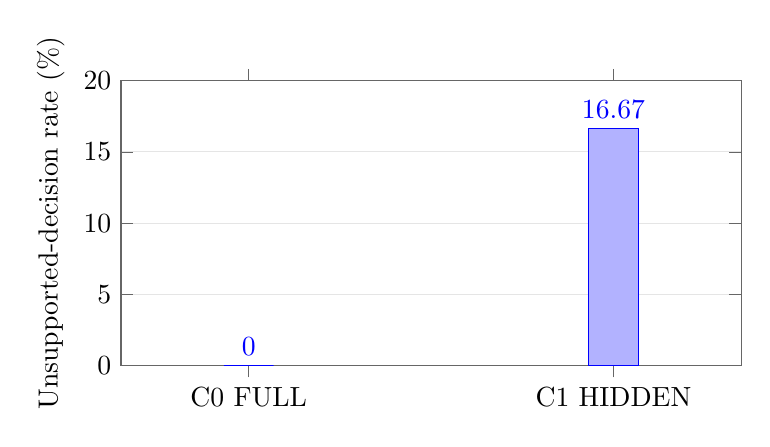
\begin{tikzpicture}
\begin{axis}[
  ybar,
  ymin=0, ymax=20,
  width=0.78\linewidth,
  height=5.2cm,
  ylabel={Unsupported-decision rate (\%)},
  symbolic x coords={C0 FULL,C1 HIDDEN},
  xtick=data,
  bar width=18pt,
  nodes near coords,
  nodes near coords align={vertical},
  enlarge x limits=0.35,
  ymajorgrids=true,
  grid style={black!10},
  axis line style={black!60},
  tick style={black!60},
  fill=black!22,
  draw=black
]
\addplot coordinates {(C0 FULL,\CzeroUDR) (C1 HIDDEN,\ConeUDR)};
\end{axis}
\end{tikzpicture}

\caption{\textbf{Paired evidence-visibility intervention.} World truth and the downstream
policy are fixed; only the designated mandatory item is hidden in C1. The aggregate effect
is heterogeneous across task families (Figure~\ref{fig:family}).}
\label{fig:primary}
\end{figure}

\subsection{The direct effect is concentrated in override/invalidation}

The aggregate effect hides extreme family heterogeneity. F1--F5 each remain at 0/30 UDR
under the direct C1 intervention, while F6 rises from 0/30 to 30/30.

\begin{figure}[t]
\centering
% Frozen direct-treatment family UDR.
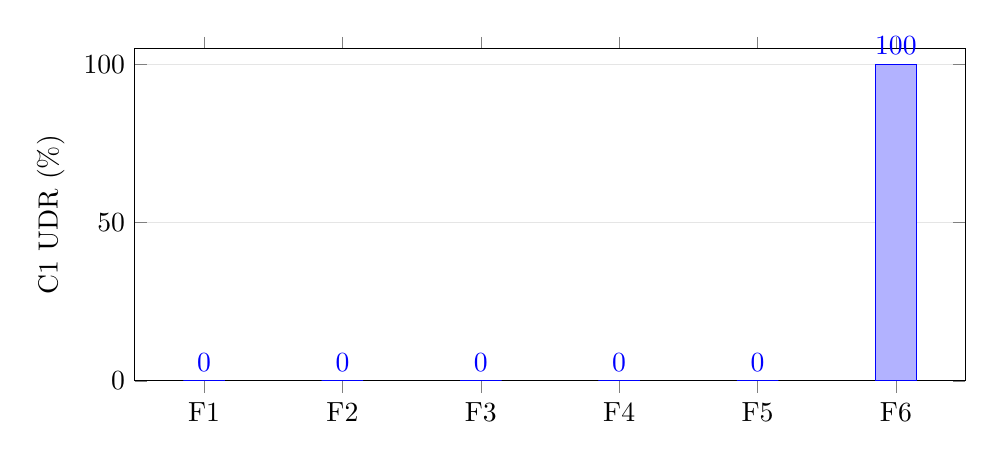
\begin{tikzpicture}
\begin{axis}[
  ybar,
  ymin=0, ymax=105,
  width=\linewidth,
  height=5.8cm,
  ylabel={C1 UDR (\%)},
  symbolic x coords={F1,F2,F3,F4,F5,F6},
  xtick=data,
  bar width=15pt,
  nodes near coords,
  nodes near coords align={vertical},
  ymajorgrids=true,
  grid style={black!10},
  fill=black!22,
  draw=black
]
\addplot coordinates {
  (F1,\FoneCOne)
  (F2,\FtwoCOne)
  (F3,\FthreeCOne)
  (F4,\FfourCOne)
  (F5,\FfiveCOne)
  (F6,\FsixCOne)
};
\end{axis}
\end{tikzpicture}

\caption{\textbf{Direct-treatment heterogeneity.} F1--F5 retain a policy-visible gap cue
after the single designated item is removed and therefore trigger conservative fallback.
In F6, the later override/invalidation disappears completely while the older instruction
remains locally actionable. The 100\% F6 rate is a mechanism result for this frozen
policy--benchmark pair, not a real-world prevalence estimate.}
\label{fig:family}
\end{figure}

The direct experiment therefore does not support the statement that any missing mandatory
evidence is dangerous. It supports the narrower mechanism claim that an otherwise
conservative visible-gap policy can fail when superseding evidence disappears without
leaving a detectable trace.

\subsection{Frozen retrievers induce broader unsupported-decision patterns}

\begin{table}[t]
\centering
\small
\begin{tabular}{lrrrrr}
\toprule
Condition & Recall & Complete & UDR & Decisive & Safe decisive \\
\midrule
C0 FULL & 100.00 & 100.00 & 0.00 & 100.00 & 100.00 \\
C1 HIDDEN & 16.67 & 0.00 & 16.67 & 16.67 & 0.00 \\
C2 Lexical & \LexRecall & \LexCoverage & \LexUDR & \LexDecisive & \LexSafeDecisive \\
C3 Hash-dense & \HashRecall & \HashCoverage & \HashUDR & \HashDecisive & \HashSafeDecisive \\
C4 Hybrid & \HybridRecall & \HybridCoverage & \HybridUDR & \HybridDecisive & \HybridSafeDecisive \\
C5 Coverage-aware & \HybridRecall & \CoverageCoverage & \CoverageUDR & \CoverageDecisive & \CoverageSafeDecisive \\
\bottomrule
\end{tabular}
\caption{Aggregate P2 results, in percent. C1 required-fact recall is a mean over all
required facts; complete coverage is 0/180.}
\label{tab:aggregate}
\end{table}

Under C2--C4, UDR ranges from 29.44\% to 33.89\%. Top-$k$ retrieval can omit combinations
of evidence rather than exactly one preregistered target, and the family pattern broadens:
F1, F2, F4, and F6 show unsupported decisions under at least one frozen retriever.

\begin{table}[t]
\centering
\small
\begin{tabular}{lrrrr}
\toprule
Family & Lexical & Hash-dense & Hybrid & Coverage-aware \\
\midrule
F1 constraint & \FoneLex & \FoneHash & \FoneHybrid & 0 \\
F2 authority & \FtwoLex & \FtwoHash & \FtwoHybrid & 0 \\
F3 temporal & \FthreeLex & \FthreeHash & \FthreeHybrid & 0 \\
F4 conflict & \FfourLex & \FfourHash & \FfourHybrid & 0 \\
F5 outcome/revision & \FfiveLex & \FfiveHash & \FfiveHybrid & 0 \\
F6 override/invalidation & \FsixLex & \FsixHash & \FsixHybrid & 0 \\
\bottomrule
\end{tabular}
\caption{Family-level UDR (\%) for the retrieval conditions. Silentness is a property of
the resulting evidence surface relative to the policy, not a synonym for the F6 label.}
\label{tab:family-retrieval}
\end{table}

\subsection{Aggregate recall is not a strict monotonic safety surrogate}

Hash-dense yields 57.22\% mandatory-fact recall and 33.89\% UDR; hybrid yields 60.00\%
recall and 29.44\% UDR; lexical yields 63.06\% recall and 31.11\% UDR. The preregistered
directional gate passes within its 2 percentage-point tolerance, but strict monotonicity
fails: lexical has higher recall than hybrid and also 1.67 percentage points higher UDR.

\begin{figure}[t]
\centering
% Three frozen retrieval conditions only. No fitted line by design.
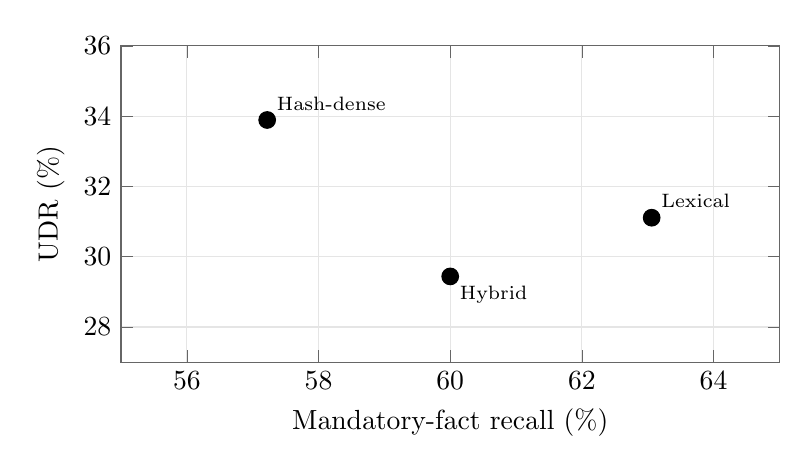
\begin{tikzpicture}
\begin{axis}[
  width=0.82\linewidth,
  height=5.6cm,
  xmin=55, xmax=65,
  ymin=27, ymax=36,
  xlabel={Mandatory-fact recall (\%)},
  ylabel={UDR (\%)},
  grid=both,
  grid style={black!10},
  axis line style={black!60},
  tick style={black!60}
]
\addplot[
  only marks,
  mark=*,
  mark size=3pt,
  black
] coordinates {
  (\HashRecall,\HashUDR)
  (\HybridRecall,\HybridUDR)
  (\LexRecall,\LexUDR)
};
\node[anchor=south west,font=\scriptsize] at (axis cs:\HashRecall,\HashUDR) {Hash-dense};
\node[anchor=north west,font=\scriptsize] at (axis cs:\HybridRecall,\HybridUDR) {Hybrid};
\node[anchor=south west,font=\scriptsize] at (axis cs:\LexRecall,\LexUDR) {Lexical};
\end{axis}
\end{tikzpicture}

\caption{\textbf{Aggregate recall is not a strict safety surrogate.} Three frozen
retrievers are shown without a fitted trend line. The data support a qualified directional
relationship, not a universal monotonic law.}
\label{fig:recall}
\end{figure}

Aggregate recall loses information about \emph{which} obligation disappeared and whether
the resulting absence is detectable by the downstream policy.

\subsection{Coverage awareness changes behavior on an identical surface}

C5 receives the identical retrieved evidence as C4 and only one additional bit indicating
whether all formal obligations are covered. C4 has UDR 53/180 = 29.44\%. C5 has UDR
0/180 while remaining decisive on all \HybridCompleteCount/\PtwoN cases with complete
formal coverage.

\begin{figure}[t]
\centering
% Same frozen retrieval surface: C4 and C5.
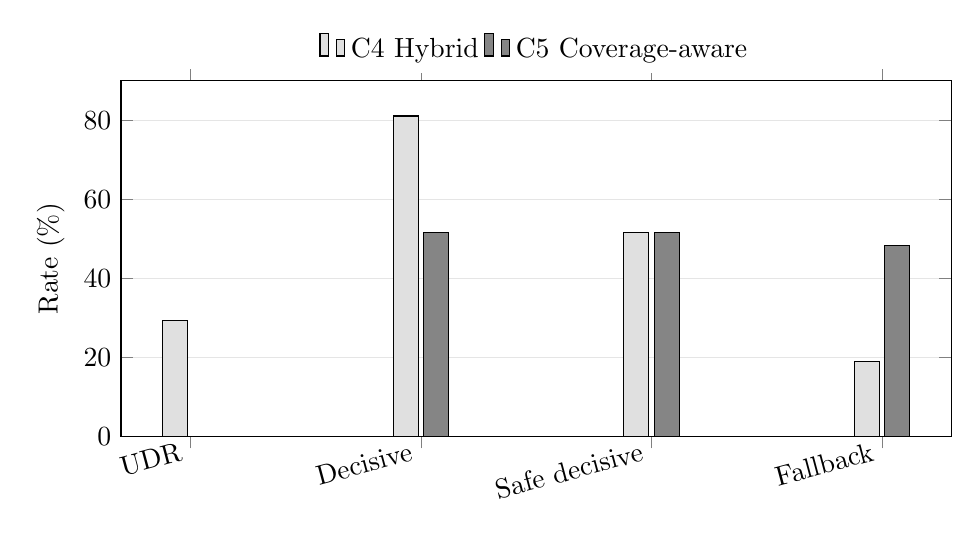
\begin{tikzpicture}
\begin{axis}[
  ybar,
  ymin=0, ymax=90,
  width=\linewidth,
  height=6.1cm,
  ylabel={Rate (\%)},
  symbolic x coords={UDR,Decisive,Safe decisive,Fallback},
  xtick=data,
  x tick label style={rotate=15,anchor=east},
  bar width=9pt,
  ymajorgrids=true,
  grid style={black!10},
  legend style={at={(0.5,1.02)},anchor=south,legend columns=2,draw=none}
]
\addplot[draw=black,fill=black!12] coordinates {
  (UDR,\HybridUDR)
  (Decisive,\HybridDecisive)
  (Safe decisive,\HybridSafeDecisive)
  (Fallback,\HybridFallback)
};
\addplot[draw=black,fill=black!48] coordinates {
  (UDR,\CoverageUDR)
  (Decisive,\CoverageDecisive)
  (Safe decisive,\CoverageSafeDecisive)
  (Fallback,\CoverageFallback)
};
\legend{C4 Hybrid,C5 Coverage-aware}
\end{axis}
\end{tikzpicture}

\caption{\textbf{Same-surface coverage-aware mitigation.} C4 and C5 share the identical
frozen hybrid retrieval surface (60.00\% mandatory-fact recall; 93/180 complete-coverage
cases). C5 adds only the completeness bit. Zero UDR here establishes sufficiency of this
information under the formal benchmark; it does not establish that a reliable coverage
signal is available in open-world deployment.}
\label{fig:coverage}
\end{figure}

C5 does not obtain zero UDR by refusing every case. Its decisive rate is 51.67\%, exactly
the 93 complete-coverage cases; the remaining 87 cases fall back. The result should be read
as a mechanism test: the downstream policy need not receive the missing evidence content
to avoid this measured failure, but it does need trustworthy information that an obligation
is uncovered.


\section{Discussion}
\label{sec:discussion}

\subsection{Missing evidence is not the same as unknowably missing evidence}

The contrast between F1--F5 and F6 shows why missing evidence is too coarse a safety
category. The same formal condition---an obligation is uncovered---has different downstream
consequences depending on whether the remaining surface advertises the gap.

At minimum, risk depends jointly on (i) which obligation is missing, (ii) whether the
remaining surface exposes that omission, (iii) how the downstream policy responds to
visible gaps, and (iv) whether a separate coverage signal exists. This also explains why
aggregate mandatory-fact recall is not strictly monotonic with UDR across C2--C4.

\subsection{Superseding evidence creates an asymmetric omission}

Override and invalidation records are asymmetric: a later record can cancel the
actionability of an earlier one. If the later record is omitted, the older record does not
necessarily look incomplete. It can look \emph{more} coherent because the contradiction
has disappeared. This differs from many ordinary missing-fact cases, where the remaining
surface can still expose a hole.

This motivates treating superseding evidence as a first-class safety obligation in
long-lived decision systems. The relevant question is not only whether an old record is
stale, but whether the system can establish that all state-changing records required to
authorize a current decision have been surfaced.

\subsection{Relation to stale-memory and revocation-enforcement failures}

The nearest prior work sharpens rather than erases our boundary. STALE shows that an agent
may have access to later evidence yet fail to infer that an older belief is no longer valid
\citep{chao2026stale}. Revocation-enforcement work shows that a memory backend may return a
record even after it has been explicitly marked revoked \citep{shen2026revoked}. Both are
important, but both retain some representation of the update or revocation in the relevant
state or retrieval path.

Our controlled F6 intervention removes the later override/invalidation from the
decision-visible surface. The older instruction then need not be contradictory,
stale-marked, or revoked-marked from the policy's perspective. The failure is one of
\emph{missing transition evidence}, not merely incorrect adjudication of visible
transition evidence.

This also changes the mitigation boundary. A better state resolver helps when the update is
visible. A revocation filter helps when an invalid record is explicitly marked as such.
Obligation coverage addresses the complementary question: has the evidence acquisition
layer surfaced the classes of evidence required to justify a consequential decision?

\subsection{Mechanism identification, not prevalence estimation}

The benchmark deliberately constructs controlled worlds and a deterministic policy so
evidence visibility can be intervened on without stochastic model confounds. This gives
strong internal control but narrow external scope. The +16.67 percentage-point aggregate
effect is not a claim that 16.67\% of real agent decisions fail this way, and the 100\% F6
direct-treatment rate is not a field prevalence estimate.

The contribution is a reproducible mechanism demonstration and boundary characterization:
under a fixed policy with explicit visible-gap checks, some obligation omissions are
self-revealing and others are not; top-$k$ retrieval can turn additional families into
silent surfaces; and independently supplied completeness information changes behavior on
the same retrieved content.

\subsection{Why obligation coverage differs from policy confidence}

A policy-confidence score asks how confident the policy is \emph{given the evidence it
received}. Silent omission is precisely a case in which the received evidence can be
locally coherent enough to support high confidence.

An obligation-coverage interface asks a different question: whether the evidence
acquisition layer satisfied a predeclared set of evidence requirements. A practical
architecture may therefore need to separate:
\begin{enumerate}
  \item retrieval relevance---which records appear useful;
  \item obligation coverage---whether required evidence classes are represented; and
  \item decision policy---what action is justified given the covered evidence.
\end{enumerate}

\subsection{C5 moves rather than solves the hard problem}

The central limitation of C5 is also the next research problem. In the benchmark,
\texttt{coverage\_complete} is computed from a frozen formal world specification. Real
systems rarely possess an oracle inventory of every fact that ought to exist.

The next technical problem is therefore not simply to add a boolean. It is how to
construct trustworthy evidence obligations and coverage monitors from schemas, workflows,
policies, provenance graphs, temporal update channels, or learned detectors without
reintroducing silent failure at the monitoring layer. A coverage monitor can itself fail
silently; false-complete and false-incomplete signals must be studied before any deployment
claim.

\subsection{Why P3 is not required for the present claim}

The confirmatory claim concerns a compositional property of a frozen evidence surface and a
frozen downstream policy. P2 identifies that mechanism through controlled evidence
interventions with no stochastic model confound. A model-based replication could test
whether similar failure modes occur in independently chosen LLM policies, but it is not
required to establish the narrower deterministic causal result reported here.

If a later P3 replication is run, model identities and prompts must be frozen before
outputs and the results must remain a replication layer rather than a retroactive
modification of P2.


\section{Threats to Validity and Limitations}
\label{sec:limitations}

\paragraph{Synthetic formal benchmark.}
The 180 scenarios are constructed from formal world specifications. This enables exact
paired interventions, dual validation, and contract-level supportedness claims, but not
human-preference or ecological-validity claims.

\paragraph{Deterministic policy.}
The confirmatory study uses one frozen deterministic policy. This isolates the
evidence-surface mechanism but does not establish prevalence across LLM agents or other
decision policies.

\paragraph{Family and policy construction.}
The direct C1 effect is concentrated entirely in F6. The frozen policy was intentionally
designed with explicit visible-gap fallbacks for several other obligation types, so this
heterogeneity is partly a property of the policy--benchmark pair. The result identifies a
controlled mechanism; it does not estimate how often each failure type occurs in deployed
agents.

\paragraph{Formal obligation oracle.}
C5 receives an accurate completeness signal derived from the benchmark's formal
obligations. Producing such a signal robustly in open-world systems remains unresolved.

\paragraph{Retriever realism.}
C2 is a lexical baseline; C3 is a deterministic hash-vector baseline rather than a
pretrained semantic encoder; C4 is their fixed reciprocal-rank fusion. These are controlled
retrieval mechanisms, not claims about state-of-the-art retrieval. All use frozen
top-$k=2$; different budgets may alter coverage and failure patterns.

\paragraph{Inferential scope.}
McNemar and bootstrap results summarize the paired 180-scenario benchmark under its frozen
construction. The scenarios are not a probability sample from a defined real-world
population, so the p-value and interval must not be interpreted as population-prevalence
estimates.

\paragraph{Coverage-signal errors are not studied.}
C5 assumes that the signal itself is correct. False-complete coverage is likely the most
safety-relevant next failure mode.

\paragraph{No deployment claim.}
The results do not establish safety in real decision-making systems or high-stakes domains.


\section{Reproducibility}
\label{sec:repro}

The study was preregistered before P2 outcomes. The 180 formal samples, dual validators,
treatment contract, downstream policy, retrievers, top-$k$, hash dimension, RRF constant,
primary endpoint, McNemar test, bootstrap procedure, seed, and formal gates were frozen
before the confirmatory run.

P2 contains \PtwoEvaluations{} deterministic evaluations across six conditions and uses
zero provider/model calls and zero cash cost. The authoritative result artifact is
\texttt{research/evidence-surface-v1/p2/out/p2-results.json}, frozen at blob SHA
\texttt{e8a749a6707dbf4614b20ef6248f81eb43dd89d4}. The figure-value macros in this paper
record that exact source SHA.

The reported P2 results were produced by replaying the frozen GitHub artifacts and frozen
JavaScript logic in a V8 execution environment. A repository-local Node replay remains
desirable as a runtime-equivalence check. Such a replay cannot alter the frozen samples,
policy, retriever parameters, statistical rules, gates, or reported outcomes.

\section{Conclusion}
\label{sec:conclusion}

A downstream safety policy can only reason about the evidence it can see. In our formally
specified synthetic benchmark, hiding a required item raises unsupported decisive behavior
from 0\% to 16.67\%, but the effect is not generic: it is concentrated in
override/invalidation cases where the omitted superseding record leaves no visible trace
that anything is missing. Frozen top-$k$ retrieval produces UDRs near 30\%, and aggregate
mandatory-fact recall is not a strictly monotonic safety surrogate.

On an identical hybrid retrieval surface, a one-bit evidence-obligation completeness
signal removes the measured unsupported decisions while preserving decisive behavior
whenever formal coverage is complete. This does not imply that reliable coverage monitoring
is easy. It isolates the architectural requirement: systems that place safety checks
downstream of retrieval need a way to distinguish the visible evidence looking sufficient
from the required evidence obligations actually being covered.

The next research problem is therefore not only better retrieval. It is trustworthy
evidence-obligation accounting under open-world, changing state.


\bibliographystyle{plainnat}
\bibliography{references}

\end{document}
